\section{Introduction}
\label{ssec:formalsem}
A benefit of employing coordination languages in general and Reo in particular is that they express the coordination patterns explicitly and separate them from the computational part of the code. This opens up possibilities for performing various types of analysis and automation such as model checking, code generation, automated test generation, etc. 

To be able to perform such tasks, it is insufficient to describe the behavior of Reo models in a verbal manner. We need a more rigorous way to unambiguously specify semantics of Reo models.% It is also desirable to be able to automatically reason about Reo.

Several formal semantics have been proposed in the recent years that express the behavior
of Reo connectors.  
Jongmans et al. \cite{sung30semantics} present a comprehensive overview of thirty models. They grouped these models into the following categories: 
\begin{itemize}
 \item \emph{Coalgebraic models}:  Two coalgebraic semantics of Reo, Timed Data Streams \cite{ABTArbab} \cite{Arbab02acoinductive} \cite{comconjan} and Record Streams \cite{izadirecasting} \cite{Izadibuchi} rely on the coalgebraic concept of \emph{stream}, which refers to an infinite sequence of elements of a given set. This class of semantics are difficult to use for analysis purpose, for instance, as an underlying model to apply model checking techniques \cite{sung30semantics}.%chera????

 \item \emph{Automata-based semantics}: A big number of Reo operational semantics are based on automata. States in these automata correspond to the states of a Reo network, while the transitions denote I/O operations. 

A list of automata based semantics for Reo are: port automata (PA) \cite{KC09},
Constraint Automata \cite{BaierCA},
 Labeled Constraint Automata (LCA) \cite{Kppelholz2009688}, Timed Constraint Automata (TCA) \cite{Arbab07MTLTCC},
 Probabilistic Constraint Automata \cite{Baier2005},
 Quantitative Constraint Automata (QCA) \cite{ArbabCMM07} \cite{qosdriven},
 Continuous Time Constraint Automata (CTCA) \cite{baier2006},
Resource Sensitive Timed Constraint Automata (RSTCA) \cite{resMengA07},
Transactional Constraint Automata (TNCA) \cite{ArMengA10}, 
Behavioral Automata (BA) \cite{JoseThesis},
Buchi Automata \cite{izadirecasting} \cite{Izadibuchi}  \cite{KULeuven217958} \cite{Izadibuchi},
Guarded Automata \cite{Bonsangue2012685} \cite{ReoAutomata},
Stochastic Guarded Automata \cite{yjmfolks} \cite{MoonSKA14}, 
Intentional Automata \cite{davidtez},
Quantitative Intentional Automata \cite{prismyoungjoo}, and
Action Constraint Automata \cite{actionautomata}.

%The join and hide operators are defined for TCA. Moreover, their composition under language equivalent is asserted.
 \item \emph{Structural operational semantics}: Some of the semantics proposed for Reo are expressed in terms of structural operational semantics. 
 Sun Meng et al.  \cite{MengAAABR12} model Reo networks in terms of the Unifying Theories of Programming (UTP) \cite{Hoare13}. %Since UTP provides formal semantics for several languages, it facilitates the specification of similar features of various languages in a similar fashion.
A UTP design consists of predicates that express assumptions on inputs and commitments on outputs. %These predicates are similar to the pairs in timed data streams semantics of Reo.
% Later, Sun Meng et al. \cite{MengAAABR12} use the UTP semantics for model based testing by refinement and test case generation. %based on work 1 ??

Another work in this field is done by Mousavi et al. \cite{Mousavi200683}. They present a Structural Operational Semantics (SOS) for some of Reo primitives in Gordon Plotkin's style \cite{tagkey200417}. In the proposed semantics, data-flow of a Reo connector is represented by a set of rules, which pair the structure of the connector with functions that map the nodes to potentially infinite sequences of data items.
%
%Together with Khosravi et al.'s  maximal progress assertion \cite{khosravi08modeling}, context sensitivity is captured in this Reo semantics. 
%A special transition rule in this model performs the  join operation on two networks. Simulation and bisimulation are also defined for the transition systems modeled in this semantics.
%
%\subsubsection{Tile Models}

Tile Model \cite{arbab2009tile} is a more recent SOS-based formal semantics for Reo that extends Gordon Plotkin's SOS inference rules. In this model, transitions are described as movements from an initial state to a final state upon firing related triggers. 

Tile Model defines composition in three ways: 
\begin{itemize}
\item
horizontal composition that models synchronization, where the effect of one tile is a trigger for another tile, 
\item vertical composition, which is a composition occurring in time. This is when the final state of one tile matches the initial state of another tile,
\item  parallel composition that captures concurrency.
\end{itemize}
%
%Tile model aims at offering a flexible and adequate semantic for Reo as it supports states and context sensitivity in forms of three coloring semantics.
%	
%
%Finally, we observe that the Tile Model can offer a uniform setting for representing not only the ordinary execution of Reo systems but also dynamic reconfiguration strategies in the style of \cite{Arbab04RCC} \cite{arbab2009tile} \cite{BaierCA}, thus reconciling relevant aspects that were dealt with separately in previous proposals.
%

 \item \emph{Semantics based on graph-coloring}.
 Connector coloring (CC) \cite{coloring} is a formal semantics for Reo that describes the behavior of a connector by assigning different colors to its ports. 
 
 The colors designate presence or absence of data-flow. This model accounts for synchronization and context dependency. It captures context dependency by propagating negative information about the absence of data-flow inside a Reo network. %4paperTile Logic \cite{ReoTiles} extends CC by adding support for both state changes and the passing of data. 
 
%\textbf{Data-Aware Coloring Semantics} Sung et al. in \cite{sung30semantics} incorporates constraints similar to those carried by transitions in Constraint Automata into Coloring Semantics regardless of the number of the colors. This facilitates their path in establishing a formal correspondence between Constraint Automata and Coloring Semantics. 
 \end{itemize}
 %Table \ref{30semtab} from \cite{sung30semantics} categories these semantics 
%\begin{tabular}[ht]{| c | c | c | c | c |}
%Coalgebraic  & Operational  & Coloring  & Context-sensitive  & o \\
%TDS & CA  & 2C & & \\
%RS & TCA  & 3C & & \\
%& & Tile & & \\
%\end{tabular}
%
%  (Section 3.3) Probabilistic
%Two colors Continuous-time
%Three colors Quantitative
%Tile models Resource-sensitive timed
%Transactional
%Other models (Section 3.4) Context-sensitive automata
%Process algebra Buchi automata
%Constraints Guarded automata
%Petri nets  intuitionistic logic Intentional automata
%Unifying theories of programming Action constraint automata
%Behavioral automata
%Structural operational semantics
%There are several formal semantics describing the behavior of a Reo network. 

\noindent
The most important types of semantics that have influenced and provided basis for the other classes of semantics  are constraint automata and coloring semantics. These models are the underlying models of  several tools for Reo ranging from animation to testing and model checking.

 In this chapter, we present the definition and examples for Reo semantics that are relevant to this thesis. In addition, we briefly discuss the time complexity of obtaining formal semantics of a Reo network using the computation rules defined by the formal semantics.
 
%\subsection{Co-algebraic formal semantics for Reo}
%There are two co-algebraic semantics for Reo: Timed Data Streams (TDS) and Record Streams (RS) \cite{izadirecasting} \cite{IzadiBC11}. The term streams used in these models refers to an infinite sequence of elements from a given set. We denote the set of all the streams over the set $S$ as $S^{\omega}$. Streams over the set $S$ is a total function from natural numbers to $S$. In other words, 
%$$s \in S^{\omega} \Leftrightarrow \mathds{N} \shortrightarrow S.$$
%
%\textbf{Timed Data Streams}
%A Timed Data Stream is a pair of data and time streams, where time is monotonically increasing over $\mathds{R} \geq 0$. TSD semantics assigns a TDS  to each Reo node, which defines what data item at what time passes through the node. The semantics of the a Reo network is calculated by assigning TDS to all its nodes. 
%
%\textbf{Record Streams}
%A record stream describes a single execution step of a Reo network. It describes which data item passes through a node at a given point of abstract time. Unlike, TDS, Record Streams (RS) semantics disregards the exact arrival time of data items. Izadi et al. in \cite{izadirecasting} \cite{IzadiBC11} introduce an operator that transforms TDS pairs to RSs and also an operator, which transforms RSs to TDSs. They prove that the latter operator is the inverse of the former operator. Furthermore, they assert that it is not so the other way around.
%
%\subsection{An overview of Reo formal semantics}
%
%\textbf{ets} Zero-safe nets \cite{zerosafenet} is a variation of Petri nets, with two types of places: zero places and stable places. While moving from a marking to another, a zero-safe places fire until all tokens occupy stable places. In this way, there may be several firings, but the intermediate firings that have tokens in zero-safe places are unobservable.
%
%To illustrate the semantical closeness between Peets Zero-safe nets in despite of their semantical differences, 
%%Zero-safe places are used in \cite{Clarkenetreo} to prevent nodes from firing more than once during an epoch. Furthermore
%Reo and zero-safe nets are mapped into intuitionistic temporal logic \cite{Clarkenetreo}. 
%
%In addition to reasoning about the model, this facilitates a more refined behavior description of a Reo model by distinguishing between internal and external choices. More analogies between Reo and Petri nets can be found in \cite{coordforcom} \cite{integstsem}.

%Fault-based Test Case Generation for Component Connectors.  \cite{aichernig2009fault}
%Component Connectors. 
%Jan Rutten. 
%In Prakash Panangaden and Franck van Breugel, editors, Mathematical Techniques for Analyzing Concurrent and Probabilistic Systems, volume 23 of %CRM, pages 73-87. 
%AMS, 2004. \cite{comconjan}
%TODO

%\textbf{Continuous Time Constraint Automata} Continuous Time CA (CTCA) \cite{baier2006} is able to model time dependent stochastic behavior of Reo networks such as stochastic waiting time of pending read/write operations. Transitions in CTCA fall into two categories: a) interactive transitions that are CA-like transition, and b) Markovian transitions, which in place of firing sets and data constraints contain a positive number,  that, similar to Markov chains, is the rate parameter of an exponential distribution over time. 
%
%A Markovian transition specifies the occurrence of a delay of maximum $t$ time units in the state $q$ with the probability of $1 - e^{- \lambda t}$. It only fires if  the interactive transitions cannot occur at the time.  Join and hide operators on CTCA are presented in \cite{baier2006}, along with strong, weak and very weak bisimulations. The compositionality of join and hide operators under strong and weak bisimulations are asserted. 

\section{Constraint automata}
\begin{definition}[Constraint automaton \cite{BaierCA}] 
 \label{def:ca}
 A constraint automaton is a tuple $\mathcal{A}$$\ =\ $$($$Q,\ $
 $ \mathcal{N},\ $$\rightarrow,$$\ q_0)$, where 
 
 \begin{itemize}
 \item $Q$ is a set of states,
 
 \item $\N$ is a set of port names,
 
 \item $\mathord{\rightarrow} \subseteq Q \times 2^{\N} \times DC \times Q$ is a transition relation, where $DC$ is the set of data constraints over a finite data
 domain $\mathit{Data}$, 
 
 \item  $q_0 \in Q$ is an initial state.
 
 \end{itemize}

\end{definition}


We write $\longtransition{q}{N,g}{p}$ instead of $(q, N, g, p) \in \mathord{\rightarrow}$.  Table~\ref{tab:basicCA}  depicts the CA corresponding to the most common Reo elements. 

Constraint automata have a compositional nature. Therefore, the semantics of a whole model can be obtained through the \emph{composition} of the given semantics of its participant elements.

\begin{table}
 \caption{Constraint automata for basic Reo primitives}
\label{tab:basicCA}
\begin{tabular}{|c|c|c|}
\hline
 \centering
    \tikz{
        \node[state] (q) {};
        \path[transition] (q) edge [loop above] node {\parbox{1.2cm}{$
            \U{a,b},\\{d_a=d_b}$}} 
	 (q) edge [loop right] node[right] {\parbox{.6cm}{$
             \emptyset,\\ true$}} (q);
    } & 
     \tikz{
        \node[state] (q) {};
        \path[transition] (q) edge [loop above] node {\parbox{1.2cm}{$
            \U{a,b},\\ {d_a=d_b}$}} (q) edge [loop right] node[right] {\parbox{1cm}{$\emptyset,\\ true$}} (q) 
            edge [loop left] node[left] {\parbox{.6cm}{$
            \U{a},\\{true}$}} (q); 
    } & 
    \tikz{
        \node[state] (q) {};
        \path[transition] (q) edge [loop above] node {\parbox{1.2cm}{$
            \U{a,b},\\{\ true}$}} 
	 (q) edge [loop left] node[left] {\parbox{.6cm}{$
             \emptyset,\\ true$}} (q); 
    }
 \\
 %\hline
  \parbox[c]{10em}{
 \addvspace{.2cm}
 CA corresponding to \centering \tikz{
            \node[point,label=left:$a$] (A) {};
            \node[point,right of=A,label=right:$b$, node distance=8mm] (B) {};
            \draw[sync] (A) -- (B);
    }} &
   \parbox[c]{10em}{
 CA corresponding to \centering \lossysyncab
 } & 
   \parbox[c]{10em}{
  CA corresponding to \centering \syncdrainab
 }\\
 \hline
  \tikz{
        \node[state] (q) {};
        \path[transition] (q) edge [loop above] node {\parbox{1.2cm}{$
            \U{a,b},\ \\{\ true} $}} 
	 (q) edge [loop left] node[left] {\parbox{.6cm}{$
             \emptyset,\ \\ true $}} (q); 
    } &
  \tikz{
        \node(alaki){};
        \node[state, right of=alaki, node distance=1.5cm] (q) {};
          \path[transition] (q) edge [loop above] node {$
        \U{b},\ {true} $} (q) edge [loop right] node[right] {\parbox{1cm}{$
             \emptyset,\ \\ true $}} (q) 
            edge [loop left] node[left] {\parbox{.6cm}{$
            \U{a},\ \\{\ true}  $}} (q); 
    } & 
  \tikz{
        \node[state] (q) {};
        \path[transition] (q) edge [loop right] node[right] {\parbox{1.5cm}{$
                     \U{a,b}, \\ {\mathit{expr}(d_a)} \\ {\wedge d_a=d_b} $}}
                	(q) (q) edge [loop below] node[below] {\parbox{1.5cm}{$ \ \ \U{a},\\{\ \ \ \neg \mathit{expr}(d_a)}$}} (q) (q) 
            edge [loop above] node[above] {\parbox{.6cm}{$
            \emptyset,\ {\ true}  $}} (q); 
    }
 \\
    \parbox[c]{10em}{
 CA corresponding to \centering {\syncspoutab}
 } & 
    \parbox[c]{10em}{
 CA corresponding to \centering {\asyncspoutab}
 } & 
 \parbox[c]{10em}{
    CA corresponding to \centering {\filterwithpredicateab} \vspace*{.1cm}
 }
 \\
 \hline
  \tikz{
        \node[state] (q) {};
        \path[transition] (q) edge [loop above] node[above] {\parbox{1.5cm}{$\U{a,b},\\{d_b=f(d_a)}$} } (q)
                                 (q) 
            edge [loop left] node[left] {\parbox{.6cm}{$
            \emptyset,\ \\{\ true}  $}} (q); 
    } & 
 \tikz{
        \node[state] (q) {};
        \node[state,right of=q, node distance=1.8cm] (p) {};
        \path[transition] (q)  edge [bend left]  node[above] {\parbox{.6cm}{$ \U{a},\\ {d_a=d} $}} (p)
           (p) edge [bend left]  node[below] {\parbox{.6cm}{$ \U{b},\\ {d_b=d} $}} (q)
           (q)  edge [loop below] node[left] {\parbox{.5cm}{ $\emptyset,\\{\ true} $}} (q)
            (p)  edge [loop below] node[right] {\parbox{.5cm}{$ \emptyset,\\{\ true} $}} (p);
    } &
  \tikz{
        \node[state] (q) {};
        \path[transition] (q) edge [loop above] node[above] {\parbox{1.5cm}{$\U{a,b,c}, \\ {d_a=d_b=d_c} $}} (q)
                              (q) 
            edge [loop left] node[left] {\parbox{1.2cm}{$
            \emptyset,{\ true\ \ } $}} (q); } 
 \\
 \parbox[c]{10em}{
    CA corresponding to \centering {\transformerwithfunctionab}
} & 
 \parbox[c]{10em}{
    CA corresponding to \centering {\fifoab}
 } & 
  \parbox[c]{10em}{
    CA corresponding to \centering {\replicatorNodeabc} \vspace*{.1cm}
 }
 \\
 \hline
 \tikz{
        \node[state] (q) {};
        \path[transition] (q) edge [loop above] node[above] {\parbox{1.2cm}{$
                     \U{a,b}, \\ {d_a=d_b} $}}
                	(q) (q) edge [loop below] node[below]{\parbox{1.2cm}{$ \U{a,c},\\{d_a=d_c}$}} (q) (q) 
            edge [loop right] node[right] {\parbox{.6cm}{$
            \emptyset,{\ true}  $}} (q); } &
    \tikz{
        \node[state] (q) {};
        \path[transition] (q) edge [loop above] node[above] {\parbox{2cm}{$\U{a,b,c}, \\ {d_c=<d_a,d_b>} $}} (q)
                              (q) 
            edge [loop left] node[left] {\parbox{.6cm}{$
            \emptyset,\ \\{\ true}  $}} (q); 
    } & 
     \\
 \parbox[c]{10em}{
    CA corresponding to \centering {\routerNodeabc} \vspace*{.1cm}
 } & 
\parbox[c]{10em}{
    CA corresponding to \centering {\mergerNodeNamedabc} \vspace*{.1cm}
 } & \\
 \hline
\end{tabular}
\end{table}

Following is the definition of the \emph{product} operator, which performs the composition.

\begin{definition}[Product on constraint automata]
 \label{def:caprod}

The product of constraint automata $\A_1=(Q_1, \N_1,\ \rightarrow_1, q_{0,1})$ and $\A_2=(Q_2, \N_2,\ \rightarrow_2, q_{0,2})$ is defined as: 
\[\A_1 \bowtie \A_2 = (Q_1 \times Q_2, \N_1 \cup \N_2, \rightarrow, q_{0,1} \times q_{0,2})\] where the following rules define the transition relation $\rightarrow$:

$$\frac{\longtransition{q_1}{N_1,g_1}{p_1},\longtransition{q_2}{N_2,g_2}{p_2},N_1\cap \N_2=N_2\cap \N_1}{\longtransition{<q_1,q_2>}{N_1\cup N_2,g_1\wedge g_2}{<p_1,p_2>}}$$

$$\frac{\longtransition{q_1}{N_1,g_1}{p_1},N_1\cap \N_2=\emptyset}{\longtransition{<q_1,q_2>}{N_1,g_1}{<p_1,q_2>}}$$

$$\frac{\longtransition{q_2}{N_2,g_2}{p_2},\N_1\cap N_2=\emptyset}{\longtransition{<q_1,q_1>}{N_2,g_2}{<q_1,q_2>}}$$   
%and$x=\frac{1+y}{1+2z^2}$
\end{definition}

We can abstract from the data-flow on certain Reo nodes using the \emph{hiding} operator defined as follows:

\begin{definition}[Hiding on constraint automata]
 \label{def:cahid}
 Let $\A=(Q, \N,\ \rightarrow, q_{0})$ be a CA and $C \in \N$. 
 
 The constraint automaton that results from hiding the node $C$ in automaton $\mathcal{A}$ is
$\exists C \left[\mathcal{A}\right] = (Q, \N \backslash \{C\},\ \rightarrow_C, q_{0})$ and the transition relation $\longrightarrow_C$ is defined as follows:

$$\dfrac{\longtransition{p}{N,g}{q}, N' = N \backslash \{C\}, g' = \exists C\left[g\right]}{p~ {\xrightarrow{N',g'}_{C}} ~q},\text{ where }$$ 

$$ \exists C \left[g\right] = \underset{d \in \mathcal{D}}{\bigvee} g\left[d\left(C\right)\slash d\right].$$
\end{definition}

\begin{BehExample}
\label{ex:contextsenmslnn}
Figure \ref{fig:calosfif} depicts the CA semantics of the Reo network of Figure \ref{fig:lossyfifo}. According to CA, it is possible that the \emph{lossySync} channel loses the incoming data in the state $q$,  where the \emph{FIFO$_1$} channel is empty. This is an example of undesired behavior that is the result of the fact that CA is not a context-dependent semantics. %???
 %depicts a Reo network that consists of a \emph{lossySync} channel and a \emph{FIFO$_1$} channel connecting on the node $b$.

   \begin{figure}[!h]
   \mesallossyfif    
    \caption{A context-dependent Reo connector}
    \label{fig:lossyfifo}
   \end{figure}  
       \begin{figure}[!h]
\centering
   \vspace{.2cm}
   \begin{tikzpicture}[node distance=2.8cm, bend angle=35,auto,baseline=(q.base)]
     %\tikz{%TCA for the \emph{timer} channel with early expiration
		\node[state,initial] (q) {$q$};
		\node[state,right of=q, node distance=3cm] (p) {$p$}; %{\parbox{1.25cm}{$\ $}};
		\path[transition] (q) edge [bend left] node[above,pos=.6] {\parbox{6.2cm}{$\ \ \ \{a, b_1, b_2\}, d(a)=d(b_1) \wedge d(b_2)=d(c)$} } (p)  
		                  (q) edge [loop below] node[left,pos=.4] {$\{a\}, true\ $} (q)
		                  (p) edge [bend left] node[below,pos=.5] {$\{a, c\}$, true} (q)
		                  (p) edge [loop below] node[right,pos=.4] {$\{a\}, true$} (p)
		                  (p) edge [] node[above,pos=.5] {$\{c\}, true$} (q); {A}
	      %}
    \end{tikzpicture}
    \caption[CA of Figure \ref{fig:lossyfifo}]{Constraint automaton of the Reo network of Figure \ref{fig:lossyfifo}}
\label{fig:calosfif}
\end{figure}

               
\end{BehExample}

\begin{BehExample}
\label{ex:contextsendo}
Figure \ref{fig:cadofilter} illustrates the CA of the Reo network of  
Figure \ref{fig:dofilters}. Since, CA is data-aware it can describes the correct behavior of this data-aware network.

%depicts a Reo network that consists of two  \emph{filter} channels with negating conditions, which connect on the node $b$.

   \begin{figure}[!h]
   \centering
{\mesaldofilter}
%  \dofilterwithpredicateabc}
  \caption{A data-aware Reo connector}
    \label{fig:dofilters}
   \end{figure}      

\begin{figure}[!h]
\centering
   \begin{tikzpicture}[node distance=2.8cm, bend angle=35,auto,baseline=(q.base)]
     %\tikz{%TCA for the \emph{timer} channel with early expiration
		\node[state] (q) {$q$};
	%	\node[state,right of=q, node distance=3cm] (p) {\parbox{1.25cm}{$\ \ p(d)\\x<=t$}};
		\path[transition] %(q) edge [bend left] node[above,pos=.6] {\parbox{2cm}{$\{a\}, x:=0,\\\ \ \ d:=\hat{a}$} } (p)  
		              %    (p) edge [bend left] node[below,pos=.4] {\parbox{2.cm}{$\{b\}, x<t, \\ \hat{b}=d$} } (q)
		                  (q) edge [loop right] node[right,pos=.3] {\parbox{2.5cm}{$\{a, b_1, b_2\}, \\ d(a) =d(b_1) \wedge  \\ d(b_1)=d(b_2) \wedge \\ p(a) \wedge p(b_1)$} } (q)
		                  (q) edge [loop left] node[left,pos=.3] {\parbox{1.cm}{$\{a\}, \\ p(a)$} } (q)
		                  (q) edge [loop above] node[above,pos=.3] {\parbox{1.cm}{$\emptyset, true$} } (q)
		               %   (p) edge [] node[above,pos=.3] {\parbox{1.5cm}{$\emptyset,\ x=t$} } (q)
		               ; {A}
	      %}
    \end{tikzpicture}
    \caption[CA of Figure \ref{fig:dofilters}]{Constraint automaton of the Reo network of Figure \ref{fig:dofilters}}
\label{fig:cadofilter}
\end{figure}

%   \begin{figure}[!h]
%   \centering
%      \begin{tikzpicture}[>=stealth]
%      \draw (-.5,0) node [thin]{a};
%      \draw [->,thick,dashed] (-.3,0) -- ++(.8,0);
%      \draw ++(.6,.3) node [thin]{b};
%      \draw [thick] (.6,0) circle (3pt);
%      \draw ++(.75,.25) node [thin]{};%c
%      \draw ++(1.9,0) node [thin]{c};
%      \draw [thick](0.7,0) -- (.9,0);
%      \def\rectanglepath{-- ++(0, .1) -- ++(.5,0) -- ++(0,-.2) -- ++(-.5, 0) -- ++(0,.1) --cycle}
%      \draw [thick] (.9,0) \rectanglepath;
%      \draw [->,thick] (1.4,0) --++(.25,0);
%    \end{tikzpicture}
%    \begin{tikzpicture}[>=stealth]
%      \draw (-.5,0) node [thin]{a};
%      \draw [->,thick,dashed] (-.3,0) -- ++(.8,0);
%      \draw ++(.6,.3) node [thin]{b};
%      \draw [thick] (.6,0) circle (3pt);
%      \draw ++(.75,.25) node [thin]{};%c
%      \draw ++(1.9,0) node [thin]{c};
%      \draw [thick](0.7,0) -- (.9,0);
%      \def\rectanglepath{-- ++(0, .1) -- ++(.5,0) -- ++(0,-.2) -- ++(-.5, 0) -- ++(0,.1) --cycle}
%      \draw [thick] (.9,0) \rectanglepath;
%      \draw [->,thick] (1.4,0) --++(.25,0);
%    \end{tikzpicture}
%    \caption{A context-dependent Reo connector}
%    \label{fig:dofilters}
%   \end{figure}      
\end{BehExample}

\section{Constraint automata with state memory}
\label{sec:casm}
Constraint automata with state memory (CASM) \cite{CASMPourvatan2012} extends CA with variables that represent local memory cells of automata states. %It also explicitly distinguishes between the ports of different kinds and splits them into the disjoint sets of \emph{snk}, \emph{src}, and \emph{mix}. ???? 
Because CASM elaborates on state information, we choose to use CASM instead of CA, in our work.% the main semantic model of Reo that our framework generates. 
\begin{definition}[Constraint automaton with state memory]
 \label{def:casm}
A constraint automaton with state memory (CASM) is a tuple $A = (Q, \mathcal{N}, \rightarrow, q_0, \mathcal{M})$ where
\begin{itemize}%{\quad}{}
 \item $Q$ is a finite set of states.
 \item $\mathcal{N}$ is a finite set of names.
 \item $\rightarrow$, a finite subset of $Q \times 2^{\mathcal{N}} \times DC(\mathcal{N}, \mathcal{M}, \mathcal{D}) \times Q$, is the transition relation of $A$,  where $DC(\mathcal{N}, \mathcal{M}, \mathcal{D})$ is the set of data constraints, defined below.
 \item $q_0 \in Q$ is an initial state.
 \item $\mathcal{M}$  is a set of memory cell names, where $\mathcal{N} \cap \mathcal{M} = \emptyset. $
\end{itemize}
\end{definition}

Every $n \in \mathcal{N}$ represents a node in a Reo connector. The set $\mathcal{N}$ is partitioned into three mutually disjoint sets of source nodes $\mathcal{N}^{src}$, mixed nodes $\mathcal{N}^{mix}$, and sink nodes $\mathcal{N}^{snk}$. 

Because we make the replication and merge inherent in Reo nodes explicit as \emph{replicator} and \emph{merger} primitives, at most two primitive ends coincide on every node $n \in \mathcal{N}$. Thus, it follows that a source or a sink node contains only a single (source or sink) primitive end, and a mixed node contains exactly one source and one sink primitive ends.

We write $\longtransition{q}{N,g}{p}$ instead of $(q, N, g, p) \in \rightarrow$. For every transition $\longtransition{q}{N,g}{p}$, we require that $g \in DC(N,\mathcal{M}, \mathcal{D})$, where $\mathcal{D}$ is the global set of numerical data values and $DC(N,\mathcal{M}, \mathcal{D})$ is the language defined by the following grammar:
$$\ g \ \ ::=\ \ \emph{true}\ \ |\ \  \neg\ g\ \ |\ \ g \wedge g \ \ |\ \ u = u\ \ |\ \ u < u,\ \  $$
$$\ u \ \ ::=\ \ d(n)\ \ |\ \ m'\ \ |\ \ m\ \ |\ \ v.$$

In this grammar,
\begin{itemize}
\item $=$ is the symmetric equality relation, 
\item $<$ is a total order relation, 
\item $n \in N \subseteq \mathcal{N}$ denotes a node name, 
\item $d(n)$ represents the data item exchanged through the node $n$, 
\item  $m \in \mathcal{M}$ correspond to a memory cell in the current state, which is the source state of the transition, 
\item $m'$ stands for the memory cell $m \in \mathcal{M}$ in the next state, which is the target state of the transition, 
\item $v \in \mathcal{D}$. 
\end{itemize}


As usual, $\emph{false}$ stands for $\neg \emph{true}$, $x > y$ stands for $y < x$, and other logical operators, such as $\vee$ and $\Rightarrow$ (the implication symbol) can be built from the given operators. 


Transitions with data constraints that can be reduced to $\emph{false}$ using the Boolean laws are impossible and we omit them. A data constraint $g$ that is always \emph{true} can be left out.

 We use $\mathcal{M}_g$ to represent the set of all $m \in \mathcal{M}$ that syntactically appear as $m$ in a data constraint $g$; and $\mathcal{M'}_g$ to refer to the set of all $m \in \mathcal{M}$ that syntactically appear as $m'$ in $g$. 
 
 The valuation function $\mathcal{V}_q : \mathcal{M} \rightarrow 2^{\mathcal{D}}$ designates the set of values $\mathcal{V}_q(m)$ of a memory cell $m \in \mathcal{M}$ in a state $q \in Q$, where $\mathcal{V}_{q_0}(m) = \emptyset$ for all $m \in \mathcal{M}$. 

A transition $\longtransition{q}{N,g}{p}$ in a given constraint automaton with state memory is possible only if there exists a substitution for every syntactic element $d(n)$, $m$, and $m'$ that appears in $g$ to satisfy $g$. 

A substitution simultaneously replaces in $g$:
\begin{itemize}
\item[-] every occurrence of $d(n)$ with the data value exchanged through the node $n \in \mathcal{N}$;
\item[-] every occurrence of $m'$ of every $m \in \mathcal{M}$ with a value $v \in \mathcal{D}$;
\item[-] every occurrence $m \in \mathcal{M}$ with:
\begin{itemize}
 \item the special symbol $'\circ'$ if $\mathcal{V}_q(m) = \emptyset$,
 \item a value $v \in \mathcal{V}_q(m)$, otherwise.
\end{itemize}
\end{itemize}

The guard $g$ is satisfied if proper replacement values can be found to make $g$ \emph{true}. Making this transition, the automaton defines the valuation function $\mathcal{V}_p$ for the target state $p$, as follows:
\begin{itemize}
\item For every $m \in \mathcal{ M}'_g$, $\mathcal{V}_p(m)$ is the set of all $v \in \mathcal{D}$ whose replacements for $m'$ satisfy $g$. 
\item For every other $m \in \mathcal{M}$, $\mathcal{V}_p(m) = \emptyset$. 
\end{itemize}

%The special symbol $'\circ'$ denotes ``no value can be substituted here.'' 
A relational operator evaluates to \emph{true} only if the values of its operands are in its respective relation. Thus, any operator with one or more $\circ$ as an operand always evaluates to \emph{false}. 

We call a CASM, \emph{normalized} iff 
\begin{itemize}
\item  It does not have two states with the same set of state memory variables.
\item Every two transitions differ at least in their start states, their target states, or their sets of synchronizing ports. 
\end{itemize}

% It is easy to see that the CASMs associated with each Reo primitive is \emph{normalized}.
 For any arbitrary CASM that is not normalized, we can normalize it by 
 \begin{itemize}
\item introducing auxiliary variables, to make the set of state memory variables unique for each state, 
\item by merging the transitions that have the same start and target states and synchronize the same ports. 
\end{itemize}

In the sequel, we consider only \emph{normalized} CASMs.

Following are the definitions for \emph{product} and \emph{hiding} operations on CASM. Both definitions are adapted from \cite{BaierCA}.

\begin{definition}[Product automaton on CASM]\label{def:productCA} The product of CASMs $\A_1$ $=$ $(Q_1,\ \N_1,\ \rightarrow_1,\ q_{0,1},\ \mathcal{M}_1)$ and $\A_2$ $=$ $(Q_2, \N_2, \rightarrow_2, q_{0,2}, \mathcal{M}_2)$ is defined as: 
\[\A_1 \bowtie \A_2 = (Q_1 \times Q_2, \N_1 \cup \N_2, \rightarrow, q_{0,1} \times q_{0,2}, \mathcal{M}_1 \cup \mathcal{M}_2)\] where the following rules define the transition relation $\rightarrow$:
$$\frac{\longtransitionno{q_1}{N_1,g_1}{1}{p_1},\ \longtransitionno{q_2}{N_2,g_2}{2}{p_2},N_1\cap \N_2=N_2\cap \N_1}{\longtransition{\langle q_1,q_2 \rangle}{N_1\cup N_2,g_1\wedge g_2}{\langle p_1,p_2 \rangle}}$$
$$ \frac{\longtransitionno{q_1}{N_1,g_1}{1}{p_1},N_1\cap \N_2=\emptyset}{\longtransition{\langle q_1,q_2 \rangle}{N_1,g_1}{\langle p_1,q_2 \rangle}} \ \ \ \ \ \   
\frac{\longtransitionno{q_2}{N_2,g_2}{2}{p_2},\N_1\cap N_2=\emptyset}{\longtransition{\langle q_1,q_2 \rangle}{N_2,g_2}{\langle q_1,p_2 \rangle}}$$
%and$x=\frac{1+y}{1+2z^2}$
\end{definition} 

Similar to CA, we can abstract from the data-flow on certain Reo nodes using the \emph{hiding} operator defined as follows:

\begin{definition}[Hiding on CASM]
Let $\A=(Q, \N,\ \rightarrow, q_{0}, \mathcal{M})$ be a CASM and $C \in \N$. 

The constraint automaton that results from hiding the node $C$ in automaton $\mathcal{A}$ is
$\exists C \left[\mathcal{A}\right] = (Q, \N \backslash \{C\},\ \rightarrow_C, q_{0}, \mathcal{M})$ and the transition relation $\longrightarrow_C$ is defined as follows:


$$\dfrac{\longtransition{p}{N,g}{q}, N' = N \backslash \{C\},\ g' = \exists C\left[g\right]}{p~ {\xrightarrow{N',g'}_{C}} ~q},\text{ where }$$ $$ \exists C \left[g\right] = \underset{d \in \mathcal{D}}{\bigvee} g\left[d\left(C\right)\slash d\right].$$
\end{definition}

To facilitate our further reasoning with CASM, we provide the following definition that gives the set of state memories used in each state.

\begin{definition}[State variables]
\label{def:statevars}
Given the CASM $\A=(Q, \N,\ \rightarrow, q_{0}, \mathcal{M})$, we define the function $S : Q \rightarrow 2^{\mathcal{M}}$ as for each $\longtransition{q}{N,g}{p}$, $m \in V_{g} \Rightarrow m \in S\left(q\right)$ and 
$m' \in V_{g} \Rightarrow m \in S\left(p\right)$.
\end{definition} 

\begin{BehExample}
\label{ex:contextsencasm}
Figure \ref{fig:casmfifo2} depicts the CASM for the Reo shown network in 
Figure \ref{fig:fifo2ex}. CASM provides an explicit representation for the stored  values using  its state variables. 

      \begin{figure}[!h]
  \centering
      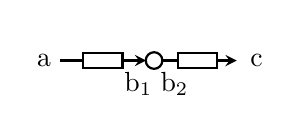
\begin{tikzpicture}[>=stealth]
      \draw (-.8,0) node [thin]{a};
    %  \draw [->,thick,dashed] (-.3,0) -- ++(.8,0);
      \draw ++(.6,.3) node [thin]{};
      \draw ++(.4,-.3) node [thin]{b$_1$\ };
      \draw ++(.8,-.3) node [thin]{\ b$_2$};
      \draw [thick] (.6,0) circle (3pt);
      \draw ++(.75,.25) node [thin]{};%c
      \draw ++(1.9,0) node [thin]{c};
      \draw [thick](0.7,0) -- (.9,0);
      \def\rectanglepath{-- ++(0, .1) -- ++(.5,0) -- ++(0,-.2) -- ++(-.5, 0) -- ++(0,.1) --cycle}
      \draw [thick] (-.3,0) \rectanglepath;
 \draw [thick](-.6,0) -- (-.3,0);
 \draw [->,thick] (.2,0) --++(.3,0);
      \draw [thick] (.9,0) \rectanglepath;
      \draw [->,thick] (1.4,0) --++(.25,0);
    \end{tikzpicture}
    \caption{FIFO$_2$}
    \label{fig:fifo2ex}
   \end{figure}   

      \begin{figure}[!h]
\centering
		  \tikz{
			\node[state, initial] (q) {\parbox[top][][c]{1cm}{$\ \ \ \ \ \ \ \ \ \ \ \ \ $}};
			\node[state, right of=q, node distance=5cm] (p) {\parbox[top][][c]{1cm}{ $\ \ \ \ m\ \ \ \ $}};
			\node[state, below of=q, node distance=3.5cm] (r) {\parbox[top][][c]{1cm} {$\ \ \ n\ \ \ $}};
			\node[state, right of=r, node distance=5cm] (s) {\parbox[top][][c]{1cm}{ $\ m,\ n \ $}};
			%transitions
			\path[transition] (q) edge [loop above] node [left] {$\emptyset, true\ $} (q); 
			\path[transition] (p) edge [loop right] node [right] {$\ \emptyset, true$} (p); 
			\path[transition] (r) edge [loop left] node [left] {$\emptyset, true\  $} (r); 
			\path[transition] (s) edge [loop right] node [right] {$\emptyset, true$} (s);
			\path[transition] (q) edge [] node [above,text width=3cm,align=center] { $\{a\},\ m'=\hat{a}$} (p);     
			\path[transition] (p) edge [bend left] node [] {$\emptyset,\ n'=m$}  (r);   
			\path[transition] (r) edge [] node [below,text width=3.5cm,align=center] {$\{a\},\ m'=\hat{a} \wedge \ n'=n$}  (s);
			\path[transition] (s) edge [] node [right] { $\{c\}, m'=m  \wedge  \hat{c}=n$}  (p);
			\path[transition] (r) edge [] node [left] {$\{c\}, \hat{c}=n$}  (q);              	
			\path[transition] (r) edge [bend left] node [] { $\{a,c\}, m'=\hat{a} \wedge \hat{c}=n$}  (p);   
		  }                 
    \caption[CA of Figure \ref{fig:fifo2ex}]{Constraint automaton of the Reo network of Figure \ref{fig:fifo2ex}}
\label{fig:casmfifo2}
\end{figure}
\end{BehExample}

\section{Constraint automata with priority}
\begin{definition}[Constraint automaton with priority]
  \label{def:pca}
 A constraint automaton with priority is a tuple $\mathcal{P} = (\mathcal{A}, \mathcal{R}, \mathcal{S}, \mathcal{T})$ where
 \begin{itemize}
  \item $\mathcal{A} = (\mathcal{Q}, \mathcal{N}, \mathcal{N}^{mix}, \mathcal{N}^{src}, \mathcal{N}^{snk}, \longrightarrow, \mathcal{Q}_{0})$ is a constraint automaton,
  \item $\mathcal{R} \subset 2^{\N}: \forall R \in \mathcal{R}$ is a subset of $\mathcal{N}$, such that if a node $n \in R$ connects to the priority imposing channel, $PrioritySync$, the priority affects $\bar{n} \in R$. 
  \item $S \subset \mathcal{R} \times \mathcal{R}$ is the set pairs of subsets of $\mathcal{N}$, such that $\forall (X, Y) \in S$, the priority imposed on the region $X$ can propagate to the region $Y$,
 \item $\mathcal{T}=^{def} (t, \triangleleft) : t \in R$ and $\triangleleft \subseteq \longrightarrow \times \longrightarrow$ is a binary relation on the transitions of A such that $\longtransition{q}{N,g}{p} \triangleleft \longtransition{\bar{q}}{\bar{N},\bar{g}}{\bar{p}}$ implies $q = \bar{q}$ and $(N, g) \neq (\bar{N}, \bar{g})$.
 \end{itemize}
\end{definition}

\begin{longtable}{|c|c|}
%\newpage
\caption{Priority constraint automata of commonly used Reo primitives} \label{tab:CAP4prims} \\
    \hline %ROW 1
          \tikz{
	      \node[state] (q) {q};
	      \path[transition] (q) edge [loop above] node {$\{a,b\},d_a=d_b$} (q);
	      \path[transition] (q) edge [loop below] node {$\emptyset,\textit{true}$} (q);
          } &
          \tikz{
          \node[state] (q) {q};
          \path[transition] (q) edge [loop above] node {$\{a,b\},d_a=d_b$} (q);
          \path[transition] (q) edge [loop below] node {$\emptyset,\textit{true}$} (q); 
                  }
\\ 
         $Q_0 = \{q\},$ & $Q_0 = \{q\},$ \\
         $R = \{\{a,b\}\},$  &   $R = \{\{a\},\{b\}\},$\\
         $S = 1,$  & $S = 1 \cup \{(\{b\},\{a\})\},$ \\
         $T  = \{\{a,b\} : $&  $T = \emptyset $\\
 $\longtransition{q}{\{a,b\},d_a=d_B}{q} \lhd \longtransition{q}{\emptyset,true}{q}\}$ & \\ 
         \parbox[c]{10em}{CAP corresponding to \centering 
          \tikz{
          	   \node[point,label=left:$a$] (A) {};
           	   \node[point,right of=A,label=right:$b$, node distance=1cm] (B) {};
           	   \draw[sync] (A) -- (B);
           	   \node[] at (.5,0) {$!$};} } & 
           	         \parbox[c]{10em}{CAP corresponding to \centering \tikz{
          	   \node[point,label=left:$a$] (A) {};
           	   \node[point,right of=A,label=right:$b$, node distance=1cm] (B) {};
           	   \draw[sync] (A) -- (B);
           	   \node[] at (.5,0) {$)$};}} \\
\hline %ROW 2
          %CAPS
          \tikz{
	      \node[state] (q) {q};
	      \path[transition] (q) edge [loop above] node {$\{a,b\},d_a=d_b$} (q);
	      \path[transition] (q) edge [loop below] node {$\emptyset,\textit{true}$} (q);
          } &
          \tikz{
          \node[state] (q) {q};
          \path[transition] (q) edge [loop above] node {$\{a,b\},d_a=d_b$} (q);
          \path[transition] (q) edge [loop below] node {$\emptyset,\textit{true}$} (q); 
                  }
         \\
         $Q_0 = \{q\},$ & $Q_0 = \{q\},$ \\
         $R = \{\{a,b\}\},$  &   $R = \{\{a\},\{b\}\},$\\
         $S = 1 \cup \{(\{a\},\{b\})\},$  & $S = 1 \cup \{(\{a\},\{b\}), (\{b\},\{a\})\},$ \\
         $T = \emptyset $  & $T  = \emptyset$ \\ 
         \parbox[c]{10em}{CAP corresponding to \centering 
 \tikz{
          	   \node[point,label=left:$a$] (A) {};
           	   \node[point,right of=A,label=right:$b$, node distance=1cm] (B) {};
           	   \draw[sync] (A) -- (B);
           	   \node[] at (.5,0) {$($};}} &
           	   \parbox[c]{10em}{CAP corresponding to \centering 
	   \tikz{
          	   \node[point,label=left:$a$] (A) {};
           	   \node[point,right of=A,label=right:$b$, node distance=1cm] (B) {};
           	   \draw[sync] (A) -- (B);
           	   \node[] at (.5,0) {$)($};} }
           	   \\ \hline
 % Row 3
\begin{minipage}[t]{.4\linewidth}
         \hspace*{1.5cm}   \tikz{
          \node[state] (q) {q};
          \path[transition] (q) edge [loop right] node {\parbox{1.2cm}{$
            \U{a,b},\ \\{\ d_a=d_b} $}} 
	 (q) edge [loop above] node[above] {\parbox{.6cm}{$
             \emptyset,\ true $}} (q); }
    \end{minipage}&
     	  \begin{minipage}[t]{.5\linewidth}
       \hspace*{1.2cm}   \tikz[y=4.80pt,x=0pt]{
          \node[state] (q) {q};
          \path[transition] (q) edge [loop above] node {\parbox{1cm}{$
            \U{a,b},\\{d_a=d_b} $}} (q) edge [loop right] node[right] {\parbox{1cm}{$
             \emptyset,\ true $}} (q) 
            edge [loop left] node[left] {\parbox{.6cm}{$
            \U{a},\ \\{\ true}  $}} (q); } 
   \end{minipage}
   \newline
   \\
         $Q_0 = \{q\},$ & $Q_0 = \{q\},$ \\
         $R = \{\{a, b\}\},$  &   $R = \{\{a, b\}\},$\\
         $S = 1,$  & $S = 1,$ \\
         $T = \emptyset $  & $T  = \{\emptyset : \longtransition{q}{\{a,b\},d_a=d_b}{q} \lhd \longtransition{q}{\{a\},true}{q}, $ \\
         & $\emptyset : \longtransition{q}{\{a, b\},d_a=d_b}{q} \lhd \longtransition{q}{\emptyset,true}{q},$ \\
          & $\emptyset : \longtransition{q}{\{a\},true}{q}, \lhd \longtransition{q}{\emptyset,true}{q}\}$ \\
        \parbox[c]{10em}{CAP corresponding to \centering 
            \tikz{
          	   \node[point,label=left:$a$] (A) {};
           	   \node[point,right of=A,label=right:$b$, node distance=8mm] (B) {};
           	   \draw[sync] (A) -- (B);}}   & 
           	   \parbox[c]{10em}{CAP corresponding to \centering 
\lossysyncab} \\
 \hline
%Row 4
     	\begin{minipage}[t]{.4\linewidth}
          \hspace*{1.5cm} \tikz{
                   \path[transition] (q) edge [loop right] node[right] {\parbox{1.2cm}{$
            \U{a,b},\ \\{\ true} $}} 
	 (q) edge [loop above] node[above] {\parbox{.6cm}{$
             \emptyset,\ true $}} (q); }
    \end{minipage}
    &
     	\begin{minipage}[t]{.5\linewidth}
       \hspace*{1.8cm} \tikz{
                  \node[state] (q) {q};
                    \path[transition] (q) edge [loop right] node[right] {\parbox{.9cm}{$
            \U{a,b},\ \\{\ true} $}} 
	 (q) edge [loop above] node[above] {\parbox{.6cm}{$
             \emptyset,\ true $}} (q); }
        
   \end{minipage} 
     \\
         $Q_0 = \{q\},$ & $Q_0 = \{q\},$ \\
         $R = \{\{a, b\}\},$  &   $R = \{\{a, b\}\},$\\
         $S = 1,$  & $S = 1,$ \\
         $T = \emptyset $  & $T  = \emptyset$
   \\
   \parbox[c]{10em}{CAP corresponding to \centering 
  {\syncdrainab} \vspace*{.1cm}} &
  \parbox[c]{10em}{CAP corresponding to \centering {\syncspoutab} \vspace*{.1cm}}
  \\
\hline
%Row 5
     	\begin{minipage}[t]{.4\linewidth}
         \centering
        \hspace*{1cm}    \tikz[y=4.80pt,x=0pt]{
          \node[state] (q) {q};
          \path[transition] (q) edge [loop above] node {\parbox{2.5cm}{$
            \ \ \ \ \ \U{b},{\ true} $}} (q) edge [loop right] node[right] {\parbox{2.5cm}{$
             \emptyset,\ true\ $}} (q) 
            edge [loop left] node[left] {\parbox{.6cm}{$
            \U{a},\\ { true}  $}} (q); } 
    \end{minipage}&
     	\begin{minipage}[t]{.5\linewidth}
         \centering
         \hspace*{1cm} \tikz[y=4.80pt,x=0pt]{
          \node[state] (q) {q};
          \path[transition] (q) edge [loop above] node {\parbox{1.5cm}{$
             \U{b},{\ true} $}} (q) edge [loop right] node[right] {\parbox{1.5cm}{$
             \emptyset,\ true $}} (q) 
            edge [loop left] node[left] {\parbox{.6cm}{$
            \U{a},\ \\{\ true}  $}} (q); } 

    \end{minipage}
      \\
         $Q_0 = \{q\},$ & $Q_0 = \{q\},$ \\
         $R = \{\{a, b\}\},$  &   $R = \{\{a, b\}\},$\\
         $S = 1,$  & $S = 1,$ \\
         $T = \emptyset $  & $T  = \emptyset$
    \\
           	\parbox[c]{10em}{CAP corresponding to \centering {\asyncdrainab} \vspace*{.1cm} }  & 
           		\parbox[c]{10em}{CAP corresponding to \centering {\asyncspoutab} \vspace*{.1cm} }
           	\\
\hline
%Row 6
     	\begin{minipage}[t]{.4\linewidth}
         \centering
        \tikz{ 
              	\node[state] (q) {q};
                 	\path[transition] (q) edge [loop right] node[right] {\parbox{1.5cm}{$
                     \U{a,b}, \\ {\mathit{expr}(d_a) \wedge} \\ {d_a=d_b} $}}
                	(q) (q) edge [loop left] node[left] {\parbox{1.5cm}{$ \U{a},\\{\neg \mathit{expr}(d_a)}$}} (q) (q) 
            edge [loop above] node[above] {\parbox{1cm}{$
            \emptyset,\ {\ true}  $}} (q); }
   \end{minipage} &
     	\begin{minipage}[t]{.5\linewidth}
         \centering
          \hspace*{2cm}
\tikz{
                                 \node[state] (q) {q};
                                 \path[transition] (q) edge [loop right] node[right] {\parbox{2.5cm}{$\U{a,b},\\{d_b=f(d_a)}$} } (q)
                                 (q) 
            edge [loop above] node[above] {\parbox{.6cm}{$
            \emptyset, {\ true}  $}} (q); }
   \end{minipage} 
     \\
         $Q_0 = \{q\}, R = \{\{a, b\}\},$ & $Q_0 = \{q\}, R = \{\{a, b\}\},$ \\
      %   $R = \{\{a, b\}\},$  &   $R = \{\{a, b\}\},$\\
         $S = 1, T = \emptyset $  & $S = 1, T = \emptyset $ \\
       %  $T = \emptyset $  & $T  = \emptyset$ \\
    \parbox[c]{12em}{CAP corresponding to \centering	{\filterwithpredicateab} \vspace*{.2cm}} &
    	\parbox[c]{12em}{CAP corresponding to \centering {\transformerwithfunctionab} \vspace*{.2cm}}
    \\
\hline
%&\\
   %Row 7
     	\begin{minipage}[t]{.4\linewidth}
         \centering
\hspace{-.8cm}
                \raisebox{0mm}{\tikz{
           \node[state,initial] (q) {q};
           \node[state,right of=q, node distance=1.8cm] (p) {p};
           \path[transition] (q)  edge [bend left]  node[above] {\parbox{1.6cm}{$ \U{a}, {d_a=d} $}} (p)
           (p) edge [bend left]  node[below] {\parbox{.5cm}{$ \U{b}, {d_b=d} $}} (q)
           (q)  edge [loop below] node[left] {\parbox{1cm}{ $\emptyset,{\ true}\ \ $}} (q)
            (p)  edge [loop right] node[right] {\parbox{.6cm}{$ \emptyset,{\ true} $}} (p); }}
    \end{minipage} 
    &    
     	\begin{minipage}[t]{.5\linewidth}
     	\centering
                        \tikz{
                            	\node[state] (q) {q};
                            	\path[transition] (q) edge [loop right] node[right] {\parbox{1.5cm}{$\U{a,b,c}, \\ {d_a=d_b=d_c} $}} (q)
                              (q) 
            edge [loop above] node[above] {\parbox{.6cm}{$
            \emptyset,\ {\ true}  $}} (q); }
	\end{minipage}
	  \\
         $Q_0 = \{q\},\ R = \{\{a\}, \{b\}\},$ & $Q_0 = \{q\}, R = \{\{a, b, c\}\},$ \\
        % $R = \{\{a\}, \{b\}\},$  &   $R = \{\{a, b, c\}\},$\\
         $S = 1,\ T = \emptyset $  & $S = 1,\ T = \emptyset $ \\
%         $T = \emptyset $  & $T  = \emptyset$ \\
          \parbox[c]{10em}{CAP corresponding to \centering {\fifoab}}
       &       \parbox[c]{12em}{CAP corresponding to \centering {\replicatorNodeabc} \vspace*{.1cm}}
 \\
\hline
     %Row 8
     	\begin{minipage}[t]{.4\linewidth}
        \centering    
         \tikz{
              	\node[state] (q) {q};
                 	\path[transition] (q) edge [loop right] node[right] {\parbox{1.5cm}{$
                     \U{a,b}, \\ {d_a=d_b} $}}
                	(q) (q) edge [loop left] node[left] {\parbox{1.05cm}{$ \U{a,c},\\{d_a=d_c}$}} (q) (q) 
            edge [loop above] node[above] {\parbox{.6cm}{$
            \emptyset,\ {\ true}  $}} (q); }
    \end{minipage}  	
	 &
     	\begin{minipage}[t]{.5\linewidth}
        \centering    
            \tikz{
                            	\node[state] (q) {q};
                            	\path[transition] (q) edge [loop right] node[right] {\parbox{1.5cm}{$\U{a,b,c}, \\ {d_c=<d_a,d_b>} $}} (q)
                              (q) 
            edge [loop left] node[left] {\parbox{.6cm}{$
            \emptyset,\ \\{\ true}  $}} (q); }
    \end{minipage}
         \\
         $Q_0 = \{q\},$ & $Q_0 = \{q\},$ \\
         $R = \{\{a, b, c\}\},$  &   $R = \{\{a, b, c\}\},$\\
         $S = 1,$  & $S = 1,$ \\
         $T = \emptyset $  & $T  = \emptyset$
\\           
\parbox[c]{10em}{CAP corresponding to \centering {\routerNodeabc} \vspace*{.1cm}} & 
\parbox[c]{10em}{CAP corresponding to \centering  {\mergerNodeNamedabc} \vspace*{.1cm}}\\ \hline
\end{longtable}

Observe that the nodes in $R$ connect to each other by priority propagating channels such as Sync, PrioritySync, SyncDrain. The connections of the regions paired in $S$ is, however, via priority blocking channels like BlocingSinkSync, BlockingSourceSync and AsyncDrain. The sets $\mathcal{R}$,  $\mathcal{S}$  and the tag $t$ in $\mathcal{T}$ are auxiliary concepts for composition of CAPs. Table \ref{tab:CAP4prims} shows CAPs corresponding to Reo elements.

Similar to CA, the \emph{product-automaton} operator ($\bowtie$) computes the CAP corresponding to a Reo network from CAPs of its substituent elements.

%Composition
Let $\mathcal{P}_{1}$ and $\mathcal{P}_{2}$ be the two CAPs, $\tau_{1}, \lambda_{1} \in \longrightarrow_{1}$, $\tau_{1} \triangleleft \lambda_{1}$ and $\tau_{2}, \lambda_{2} \in \longrightarrow_{2}$. If $\tau_{1}$ and $\tau_{2}$ synchronize to form a transition $\tau \in \longrightarrow_{P_{1} \bowtie P_{2}}$, $\lambda_{1}$ and $\lambda_{2}$ synchronize to form a transition $\lambda \in \longrightarrow_{P_{1} \bowtie P_{2}}$, the relation of $\tau \triangleleft \lambda$ is \emph{full lifting} of the $\tau_{1} \triangleleft \lambda_{1}$. 

Since the priority blocking channels can affect the propagation of the priority, the priority relations that full lifting defines are not always valid on the product of the automata. We need to eliminate invalid transitions that are results of improper propagation of the priority.%TODO y such as the transition ???? in Figure.

%\begin{figure}{c}
  %  \scriptsize
        %\tikz{
          %\node[state] (q) {};
          %\node[state, right of=q, node distance=5cm] (p) {m};
          %\path[transition] (q) edge [loop above] node {$\{\},\textit{true}$} (q); 
          %\path[transition] (q) edge [bend left] node {$\{a, b, e\},\hat{a}=\hat{b} \wedge \hat{b}=\hat{e} \wedge \hat{m}'=\hat{e}$}  (p);     
          %\path[transition] (q) edge [bend right] node {$\{c,d,e\},\hat{d}=\hat{e} \wedge \hat{m}'=\hat{e}$}  (p);
          %\path[transition] (p) edge [loop above] node {$\{\},\textit{true}$} (p); 
          %\path[transition] (p) edge  node {$\{f\}, \hat{m}=\hat{f}$}  (q);                            
                 % }
   %\label{fig:invalidlifting}
   %\caption{Invalid lifting}
%\end{figure}


The following three cases are the only valid propagation of the priority~\cite{priority}:
\begin{itemize}
 \item \emph{Propagation over empty transitions}: If $\lambda$ is an empty transition, then $\lambda_{1}$ and $\lambda_{2}$ are also empty transitions. In this case, full lifting brings a new priority imposition as: $\tau \triangleleft \lambda$.
 \item \emph{Propagation by containment}: If $\lambda_{1}$ is a proper transition, then $\lambda$ is a proper transitions, which contains $\lambda_{1}$. Therefore, full lifting is a natural growth of the previously imposed priority that preserves the priority relation as: $\tau \triangleleft \lambda$. 
 \end{itemize}

 \FloatBarrier

\begin{itemize} 
 \item \emph{Propagation by seepage}: If $\lambda_{1}$ is an empty transition, but $\lambda$ is a proper transition, then $\lambda_{2}$ is also a proper transition. Under this condition, full lifting is not always valid. Therefore, we need more restriction to preserve the new priority relation that full lifting impose that is $\tau \triangleleft \lambda$. The seepage relation $\mathcal{S}$ and the tag $t$ of the transition help to check the validity of full lifting for this case. So, the full lifting is valid if there exists a finite sequence of regions $r_{0},..,r_{i},r_{i+1},..,r_{n}$ such that $r_{i} \in R, (r_{i}, r_{i+1}) \in \mathcal{S}, r_{0}=t$ and  $r_{n}$ includes all nodes involved in the transition $\lambda_{2}$. Note that $\mathcal{S}$ is the seepage relation that defines the allowed propagation of the priority through regions. Observe that if $t_{1} = \emptyset$ , then $t = \emptyset$. Since $\emptyset \notin \mathcal{R}$, such a sequence does not exist and the full lifting is not valid.
\end{itemize}

Following is the definition of the CAP product operator.
\begin{definition}[Product-automaton]
Let $\mathcal{P}_{i}=(\mathcal{A}_{i}, \mathcal{R}_{i}, \mathcal{S}_{i}, \mathcal{T}_{i})$, $i=1, 2$ be two %normalized?
CAPs, where $\mathcal{A}_{i} = (\mathcal{Q}_{i}, \mathcal{N}_{i}, \mathcal{N}_{i}^{mix}, \mathcal{N}_{i}^{src}, \mathcal{N}_{i}^{snk}, \longrightarrow, \mathcal{Q}_{0,i})$, such that:
\[\mathcal{N}_{1} \cap \mathcal{N}_{2} \subseteq \mathcal{N}_{1}^{src} \cap \mathcal{N}_{2}^{snk} \cup \mathcal{N}_{1}^{snk} \cup \mathcal{N}_{2}^{src}\]
The definition of the product-automaton $\mathcal{P}_{1} \bowtie \mathcal{P}_{2} = (\mathcal{A}_{1} \bowtie \mathcal{A}_{2}, \mathcal{R}, \mathcal{S}, \mathcal{T})$ follows:

  \label{def:productcap}
\end{definition}

\vspace*{-.5cm}

\begin{lstlisting}[frame=single,caption=Calculating $\mathcal{R}$,label=arr:calcR,mathescape]
$\mathcal{R}\ :=\  \emptyset$
for each $\ r_{1}\ \in \  \mathcal{R}_{1} $
if $\exists \ r_{2} \  \in \ R_{2} \ : \ r_{1} \ \cap \ r_{2} \ \neq  \emptyset $
 $\;\; \; \; \mathcal{R} \ := \ \mathcal{R} \ \cup  \ r_{1} \ \cup \ r_{2} $
$\ else$
    $ \mathcal{R} \ := \ \mathcal{R} \  \cup \ r_{1}  $
for each $\ r_{2} \ \in \ \mathcal{R}_{2} $
$\;\;\;\;\ \ $if $\ \not \exists r_{1} \ \in \ R_{1} \ : \ r_{1} \ \cap \  r_{2} \ \neq \emptyset \ then $
   $\ \ \ \ \mathcal{R} \ = \ \mathcal{R} \ \cup \ r_{2} $
\end{lstlisting}

\begin{lstlisting}[frame=single,caption=Calculating seepage relation $\mathcal{S}$,label=arr:calcSS,mathescape]
$    \mathcal{S}\ := \ \emptyset $
for each $ (u_1, v_1) \ \in \ \mathcal{S}_1 $
$\;\;\;\; \mathcal{S} \ += \ (big(u_1),big(v_1))$
$\;\;\;\;$for each$ \ (u_2, v_2) \  \in \ \mathcal{S}_2 $
 $ \ \ \ \ \mathcal{S} \ += \ (big(u_2),big(v_2)) $
$\ \ \ \ \mathcal{S} \ += \ \mathcal{I}  $
\end{lstlisting}

%Calculating $\mathcal{S}$
%Calculating $\mathcal{T}$: 
Let $(t_1, \mathcal{\tau}_1 \triangleleft_1 \mathcal{\lambda}_1) \in \mathcal{T}_1$. The transition $\lambda_1$ is either empty or proper:
\begin{equation}
 \begin{array}{ll}
			\forall \ \tau_2 \ \in \ \longrightarrow_2 \ : \ \tau_1 \cap \tau_2 \neq \emptyset \hspace*{2cm} & \mbox{if $\lambda_1 $is empty} \\
			big(r_1) \ : \ \tau_1 \ || \ \tau_2 \ \triangleleft \ \emptyset  &  \\
			\forall \ \tau_2 \ \in \ \longrightarrow_2 \ : \ \tau_1 \cap \tau_2 = \emptyset & \\
			if \ exists \ a \ sequence \ such \ that  & \mbox{otherwise } \\
			\forall \ \tau_2 \ : \ \tau_1 \cap \tau_2 \neq \emptyset & \mbox{$\lambda_1$ is proper } \\
			\forall \ \lambda_2 \ : \ \lambda_1 \cap \lambda_2 \neq \emptyset & \\
			big(r_1) \ : \ \tau_1 \ || \ \tau_2 \ \triangleleft \ \lambda_1 \ || \ \lambda_2  &  
		\end{array}
\label{arr:calcS}
%\caption{Calculating seepage relation $\mathcal{S}$}
\end{equation}

\section{Connector coloring}
\label{sec:cc}
The connector coloring semantics \cite{coloring} denote the existence or absence of data-flow through the primitive ends by marking them with different colors. 

Let $\mathcal{C}olors$ be a set of colors. In a set of two colors, $\mathcal{C}olors = \{\flowdoc, \noflowdoc\}$, $\flowdoc$ denotes an occurrence and $\noflowdoc$ represents an absence of data-flow. Two colors are adequate to express the formal semantics of many Reo networks. However, they cannot express the semantics of context-dependent Reo networks.

Such a network presented in Example \ref{ex:contextsendo} is when the sink end of a \emph{lossySync} channel connects to an empty \emph{FIFO$_1$} channel; in this case, the semantics of this network according to the two-color set includes the case where the \emph{lossySync} loses its incoming data item, while the \emph{FIFO$_1$} channel is empty. This is an unacceptable behavior for a so-called context-dependent \emph{lossySync} channel: it must lose its incoming data only if its sink end cannot dispense it. In the sequel, when we refer to a \emph{lossySync} we mean its context sensitive version. 

The three coloring semantics, $\mathcal{C}olors = \{\flowsec, \triangleleft, \triangleright \}$, addresses this problem by propagating negative information regarding the absence of data-flow. It replaces $\noflowdoc$ with $\triangleleft$ and $\triangleright$ meaning that the associated primitive end, respectively, \emph{provides} or \emph{requires} a reason for no-flow. 

Considering that no-flow can occur only when at least one of the involved primitive ends \emph{provides} a reason for it, and that an empty \emph{FIFO$_1$} cannot \emph{provide} a reason for no-flow on its source end, the invalid behavior described above does not arise in the three coloring semantics.

\begin{definition}[Coloring]
A coloring $l : \mathcal{P} \rightarrow \mathcal{C}olors$ is a total function from the primitive ends to a set of colors. We refer to the global set of colorings as $\mathcal{L}$.
\end{definition}

\begin{definition}[Coloring composition]
The composition of colorings $l_1$ and $l_2$, denoted $l_1 \bullet l_2$, is defined as:

$\begin{array}{ll}
l_1 \bullet l_2 = \{&\\
& c_1 \cup c_2 | c_1 \in l_1, c_2 \in l_2, p_1 \in dom(c_1), p_2 \in dom(c_2),\\
& p_1 \text{ and } p_2 \text{ are the source and sink ends of a node} \ n, \\ & 
 \neg\ (\ c_1(p_1)=\triangleleft \ \wedge \ c_2(p_2)=\triangleright\ ) \\  & \hspace{-.45cm}  \}
\end{array}$
\end{definition}

\begin{definition}[Coloring table]
A coloring table over the primitive set \\ $P \subseteq \mathcal{P}$ is a set of colorings with the domain $P$.
\end{definition}

 \begin{definition}[Next function]
The next function $\eta : \mathcal{L} \times 2^{\mathcal{L}} \rightarrow 2^\mathcal{L}$ maps a pair of a coloring and a coloring table to a colorings table. %, which can succeed it. 
\end{definition}

\begin{definition}[Coloring semantics]
A coloring semantics of a Reo network is a tuple $CC = \langle \mathcal{P}, 2^\mathcal{L}, l_0, \eta \rangle$, where:
\begin{itemize}
 \item $\mathcal{P}$ is the set of primitive ends,
 \item $l_0 \in \mathcal{L}$ is the initial set of possible colorings,
 \item $2^\mathcal{L}$ is a set of colorings,
 \item $\eta$ is a next function that maps a pair of a coloring and a coloring table into a coloring table.
\end{itemize}
\end{definition}


\begin{BehExample}
\label{ex:contextsenchapter}
	Table \ref{fig:cclossyex} depicts the CC for the network shown in Figure \ref{fig:lossyfifoforcc}. The two flows described in the table correspond to the cases; i) when there is a write request of the end $a$, then the ends $a, b_1$ and $b_2$ have a flow, but the end $c$ provides a reason for no flow, ii) when there is no write request present on the end $a$, therefore the ends $a$ and $b_2$ require a reason for no flow and the ends $b_1$ and $c$ provides a reason for no flow. Since CC is context-sensitive, it can capture the semantics of the given network correctly.

\begin{figure}[!h]
    \mesallossyfif    
    \caption{A context-dependent Reo connector}
    \label{fig:lossyfifoforcc}
\end{figure}      

\begin{table}[!h]
    $ \begin{array}{|c|c|c|c|} \hline a & b_1 & b_2 &c \\ \hline
  - & - & - & \triangleright \\ \hline
      \triangleright & \triangleright & \triangleright & \triangleright\\ \hline
       \end{array}$ 
    \vspace{.5cm}
    \caption{Connector coloring semantics of the Reo network of Figure \ref{fig:lossyfifoforcc}}
    \label{fig:cclossyex}
\end{table}
\end{BehExample}

\newpage

\begin{longtable}[T]{|c|c|c|}
\caption{Connector coloring semantics of commonly used Reo primitives} \label{tab:CCprims} \\
\hline
&&\\
   % row 1 cell 1
\begin{minipage}[t]{.3\linewidth}
         \centering
       \hspace{.5cm}    \begin{tabular}{|c|c|}
		\hline
			a & b \\
		\hline
			$\times$ & $\times$ \\ 
		\hline
			$\circ$ & $\bullet$ \\ 
		\hline
			$\bullet$ & $\circ$ \\ 
		\hline
	\end{tabular}
    \newline
    \newline
                  \centering
                  CC corresponding to
      \begin{tabular}{c}
               \tikz{
          	   \node[point,label=left:$a$] (A) {};
           	   \node[point,right of=A,label=right:$b$, node distance=8mm] (B) {};
           	   \draw[sync] (A) -- (B);}
            \end{tabular}
                \end{minipage}
    &
          % row 1 cell 2
                %\hfill
         \hspace{.5cm}      \begin{minipage}[t]{.3\linewidth}
         \centering
         \begin{tabular}{|c|c|}
             \hline
               a & b \\
            \hline
              $\times$ & $\times$ \\ \hline
              $\circ$ & $\times$ \\ \hline
              $\times$ & $\circ$ \\ \hline
         \end{tabular}
         \newline
         \newline
               CC corresponding to 
{\lossysyncab} 
    \end{minipage}
 & % row 1 cell 3
\begin{minipage}[t]{.3\linewidth}
         \centering
            \begin{tabular}{|c|c|}
		\hline
			a & b \\
		\hline
			$\times$ & $\times$ \\ 
		\hline
			$\circ$ & $\bullet$ \\ 
		\hline
			$\bullet$ & $\circ$ \\ 
		\hline
	\end{tabular}
	\parbox{3.5cm}{ \vspace*{.2cm} 
        CC correspondence to \centering
                          	  {\syncdrainab}}
    \end{minipage}
 \\ \hline  % row 2 cel 1
 	&&\\
       	\begin{minipage}[t]{.3\linewidth}
            \centering
         \begin{tabular}{|c|c|}
		\hline
			a & b \\
		\hline
			$\times$ & $\times$ \\ 
		\hline
			$\circ$ & $\bullet$ \\ 
		\hline
			$\bullet$ & $\circ$ \\ 
		\hline
	\end{tabular}
	\parbox{3.5cm}{ \vspace*{.2cm} 
        CC correspondence to \centering
                          	  {\syncspoutab}\vspace{.3cm}}
	\end{minipage}
&
   % row 2 cell 2
   \begin{minipage}[t]{.3\linewidth}
         \centering
        % \vspace{.2cm}
         \centering
            \begin{tabular}{|c|c|}
		\hline
			a & b \\
		\hline
			$\times$ & $\times$ \\ 
		\hline
			$\circ$ & $\bullet$ \\ 
		\hline
			$\bullet$ & $\circ$ \\ 
		\hline
	\end{tabular}
	\parbox{3.5cm}{ \vspace*{.2cm} 
        CC correspondence to \centering
                          	  {\asyncdrainab}}
	\end{minipage}
&
          % row 2 cell 3
          \begin{minipage}[t]{.3\linewidth}
         \centering
            \begin{tabular}{|c|c|}
		\hline
			a & b \\
		\hline
			$\times$ & $\times$ \\ 
		\hline
			$\circ$ & $\bullet$ \\ 
		\hline
			$\bullet$ & $\circ$ \\ 
		\hline
	\end{tabular}
	\parbox{3.5cm}{ \vspace*{.2cm} 
        CC correspondence to \centering
                          	  {\asyncspoutab}}
	\end{minipage}
	\\ \hline
   &&\\
      %row 3 cel 1
    \begin{minipage}[t]{.3\linewidth}
         \centering
            \begin{tabular}{|c|c|}
		\hline
			a & b \\
		\hline
			$\times$ & $\times$ \\ 
		\hline
			$\circ$ & $\bullet$ \\ 
		\hline
			$\bullet$ & $\circ$ \\ 
		\hline
	\end{tabular}
	\parbox{3.5cm}{ \vspace*{.2cm} 
        CC correspondence to \centering
                          	  {\fifoab}}
	\end{minipage}
     &
      %row 2 cel 2
      \begin{minipage}[t]{.3\linewidth}
        % \vspace{.2cm}
         \centering
            \begin{tabular}{|c|c|}
		\hline
			a & b \\
		\hline
			$\times$ & $\times$ \\ 
		\hline
			$\circ$ & $\bullet$ \\ 
		\hline
			$\bullet$ & $\circ$ \\ 
		\hline
	\end{tabular}
		\parbox{3.5cm}{ \vspace*{.2cm} 
        CC correspondence to \centering
                          	  {\fifofullab}}
    \end{minipage}
          &
          % row 2 cell 3
     \\
    & &\\
    \hline
\end{longtable}


\begin{BehExample}
Table \ref{fig:dofilterccex} shows the CC of the Reo network shown in Figure \ref{fig:dofilterscc}.  %As a result of not considering data constraints in CC, using CC for describing this network leads to incorrect results.
 The absence of data constraints in the CC, %the $filter$ channels can either loose or pass their incoming data, arbitrary. This 
 leads to incorrect behavior, as shown in the first row of the table, where there is flow on both $b_1$ and $c$. 
%The two flows described in the table correspond to the cases; i) when there is a write request of the end $a$, then the ends $a, b_1$ and $b_2$ have a flow, but the end $c$ provides a reason for no flow, ii) when there is no write request present on the end $a$, therefore the ends $a$ and $b_2$ require a reason for no flow and the ends $b_1$ and $c$ provides a reason for no flow.	
	
\begin{figure}[!ht]
    \centering
    {\mesaldofilter}
    \caption{A data-aware Reo connector}
    \label{fig:dofilterscc}
\end{figure}      
   
\begin{table}[!ht]
\centering
    $ \begin{array}{|c|c|c|c|} 
   \hline
  a & b_1 & b_2 &c \\ \hline
  - & - & - & - \\ \hline
        - & - & - & \triangleright\\ \hline
       - & \triangleright & \triangleright & \triangleright\\ \hline
      \triangleright & \triangleright & \triangleright & \triangleright\\ \hline
       \end{array}$ 
    \vspace{.5cm}
    \caption{Connector coloring semantics of the Reo network of Figure \ref{fig:dofilterscc}}
\label{fig:dofilterccex}
\end{table}
\end{BehExample}

%In the following chapter???, we present a constraint based formal semantics for Reo, which deals with data and context. Therefore, it mitigates the explained problems.???  
%????
\section{Reo automata}
\label{sec:ra}
Bonsangue et al.~\cite{Bonsangue2012685} present \emph{Reo automata} (RA), an automata-based formal model, to deal with context-dependency in Reo.

Intuitively, a Reo automaton is a non-deterministic automaton whose
transitions are labeled in the form of $g|f$, where $g$ is a binary predicate, called \emph{guard}, and $f$ a set of nodes that fire synchronously. A transition can be taken only when its guard $g$ is true. 

Let $\Sigma = \{\sigma_1,...,\sigma_k\}$ be a set of nodes, $\bar{\sigma}$ be the negation of $\sigma$, and $\mathcal{B}_{\Sigma}$ be the free Boolean algebra generated by the following grammar:
$$g\ ::=\ \sigma\ \in\ \Sigma\ |\ \top\ |\ \bot\ |\ g\ \vee\ g\ |\ g\ \wedge\ g\ |\ \bar{g}$$

The above grammar produces \emph{guards}. Often $g_1 \wedge g_2$ is written as $g_1 g_2$. A natural order $\leq$ is defined between two guards $g_1$,$g_2 \in \mathcal{B}_{\Sigma}$ as
$$g_1 \leq g_2 \Rightarrow g_1 \wedge g_2 = g_1$$

The intended interpretation of $\leq$ is logical implication: $g_1 \implies g_2$. An
atom of $\mathcal{B}_{\Sigma}$ is a guard $a_1 ... a_k$ such that $a_i \in \bar{Sigma} \cup \Sigma$ with 

$$\Sigma = \{\sigma_i\ |\ \sigma_i \in \Sigma\}, 1 \leq i \leq k$$ %We can think of
%an atom as a truth assignment. We denote atoms by Greek letters α,β,... and the set of all atoms of
%BΣ by AtΣ. Given S ⊆ Σ, we define Sb∈ BΣ as the conjunction of all elements of S. For instance, for
%S = {a,b, c} we have Sb= abc.
%
%A transition in \emph{Reo automata} is labeled with a \emph{guard}, which is a Boolean predicate in disjunctive normal form expressing positive and negative information about presence or absence of I/O requests, and a \emph{firing} set that models the occurring I/O operations in the transition. 
%
%Below is the formal definition of Reo automaton.??
%
%Given two guards g1, g2 $\in B_{\Sigma}$, we define a (natural) order $\leq$ tting g1 $\leq$ g2 $=$ g1 $\wedge$ g2 = g1.The intended interpretation of $\leq$ is logical implication—g1 implies g2.
\begin{definition}[Reo automaton \cite{Bonsangue2012685}] 
 \label{def:ra}
 A Reo automaton % $\Sigma$ is a non-deterministic (and possibly partial) automaton with transition
%labels . Formally, a Reo??? emphsasis?? automaton
is a triple $(\Sigma, Q, \delta)$ where:
\begin{itemize}
 \item $\Sigma$ is the set of nodes,
 \item $Q$ is a set of states,
 \item  $\delta \subseteq Q \times \mathcal{B}_{\Sigma} \times 2^{\Sigma} \times Q$ is the transition relation such that for transitions labeled as $\mathcal{B}_{\Sigma} \times 2^{\Sigma}$ such that for each $\longtransition{q}{g|f}{p} \in \delta$:
 \begin{itemize}
  \item $g\ \leq \hat{f}$\ \ \ \ \ \ \ \ \ \ \ \ \ \ \ \ \ \ \ \ \ \ \ \ \ \ \ \ \ \ \ \ \ \ \ \ \ \ \ \ \ \ \ \ \ \ \ \ \ \  %(reactivity)
  \item $g\ \leq g'\ \leq \hat{f}.\ \forall \alpha \leq \ g'.\ \exists \ \longtransition{q}{g''|f}{p} \in \Sigma .\ \alpha \leq g''$ %(uniformity)
 \end{itemize}
 \end{itemize}
\end{definition}

%We write $\longtransition{q}{g|f}{p}$ instead of $(q, g, f, p) \in \mathord{\rightarrow}$.  
Table~\ref{tab:basicRA} depicts the Reo automata corresponding to the most common Reo elements.  

\begin{table}
 \caption{Reo automata for basic Reo primitives}
\label{tab:basicRA}
\begin{tabular}{|c|c|c|}
\hline
 \centering
    \tikz{
        \node[state] (q) {};
        \path[transition] (q) edge [loop above] node {\parbox{.8cm}{$ab|ab$}} (q);
	% edge [loop right] node[right] {\parbox{.6cm}{$
     %        \emptyset,\\ true$}} (q);
    } & 
     \tikz{
        \node[state] (q) {};
        \path[transition] (q) edge [loop above] node {\parbox{.8cm}{$
            ab|ab \\ a\bar{b}|a$}} (q) ;%edge [loop right] node[right] {\parbox{1cm}{$\emptyset,\\ true$}} (q) 
           % edge [loop left] node[left] {\parbox{.6cm}{$
            %\U{a},\\{true}$}} (q); 
    } & 
    \tikz{
        \node[state] (q) {};
        \path[transition] (q) edge [loop above] node {\parbox{.8cm}{$
            ab|ab$}} 
	 (q);% edge [loop left] node[left] {\parbox{.6cm}{$
          %   \emptyset,\\ true$}} (q); 
    }
 \\
 %\hline
  \parbox[c]{10em}{
 \addvspace{.2cm}
 RA corresponding to \centering \tikz{
            \node[point,label=left:$a$] (A) {};
            \node[point,right of=A,label=right:$b$, node distance=8mm] (B) {};
            \draw[sync] (A) -- (B);
    }} &
   \parbox[c]{10em}{
 RA corresponding to \centering \lossysyncab
 } & 
   \parbox[c]{10em}{
  RA corresponding to \centering \syncdrainab
 }\\
 \hline
  \tikz{
        \node[state] (q) {};
        \path[transition] (q) edge [loop above] node {\parbox{.8cm}{$
            ab|ab $}} 
	 (q);% edge [loop left] node[left] {\parbox{.6cm}{$
         %    \emptyset,\ \\ true $}} (q); 
    } &
  \tikz{
      %  \node(alaki){};
        \node[state, node distance=1cm] (q) {};
          \path[transition] (q) edge [loop above] node {\parbox{.8cm}{$\bar{a}b|b \\ a\bar{b}|a$}} (q); % edge [loop right] node[right] {\parbox{1cm}{$
             %\emptyset,\ \\ true $}} (q) 
           % edge [loop left] node[left] {\parbox{.6cm}{$
            %\U{a},\ \\{\ true}  $}} (q); 
    } & 
     \tikz{
        \node[state] (q) {};
        \node[state,right of=q, node distance=1.8cm] (p) {};
        \path[transition] (q)  edge [bend left]  node[above] {\parbox{.6cm}{$a|a$}} (p)
           (p) edge [bend left]  node[below] {\parbox{.6cm}{$ b|b $}} (q)
%           (q)  edge [loop below] node[left] {\parbox{.5cm}{ $\emptyset,\\{\ true} $}} (q)
 %           (p)  edge [loop below] node[right] {\parbox{.5cm}{$ \emptyset,\\{\ true} $}} (p);
    ;}
  %\tikz{
 %       \node[state] (q) {};
  %      \path[transition] (q) edge [loop right] node[right] {\parbox{1.5cm}{$
   %                  \U{a,b}, \\ {\mathit{expr}(d_a)} \\ {\wedge d_a=d_b} $}}
    %            	(q) (q) edge [loop below] node[below] {\parbox{1.5cm}{$ \ \ \U{a},\\{\ \ \ \neg \mathit{expr}(d_a)}$}} (q) (q) 
     %       edge [loop above] node[above] {\parbox{.6cm}{$
      %      \emptyset,\ {\ true}  $}} (q); 
   % }
 \\
    \parbox[c]{10em}{
 RA corresponding to \centering {\syncspoutab}
 }
 & 
    \parbox[c]{10em}{
 RA corresponding to \centering {\asyncspoutab}
 } &
  \parbox[c]{10em}{
    RA corresponding to \centering {\fifoab}
 }
 %\parbox[c]{10em}{
  %  RA corresponding to \centering {\filterwithpredicateab} \vspace*{.1cm}
% }
 \\
 &&\\
 \hline
 % \tikz{
  %      \node[state] (q) {};
   %     \path[transition] (q) edge [loop above] node[above] {\parbox{1.5cm}{$\U{a,b},\\{d_b=f(d_a)}$} } (q)
    %                             (q) 
     %       edge [loop left] node[left] {\parbox{.6cm}{$
      %      \emptyset,\ \\{\ true}  $}} (q); 
    %}
     \tikz{
        \node[state] (q) {};
        \path[transition] (q) edge [loop above] node[above] {\parbox{.8cm}{$
                     ac|ac \\ \bar{a}bc $}}
                	(q) %(q) edge [loop below] node[below]{\parbox{1.2cm}{$ \U{a,c},\\{d_a=d_c}$}} (q) (q) 
            %edge [loop right] node[right] {\parbox{.6cm}{$
            %\emptyset,{\ true}  $}}
            (q); }
 &
  \tikz{
        \node[state] (q) {};
        \path[transition] (q) edge [loop above] node[above] {\parbox{.8cm}{$ac|ac \\ bc|bc$}} (q)
                              (q) 
           % edge [loop left] node[left] {\parbox{1.2cm}{$
            %\emptyset,{\ true\ \ } $}} (q); 
            } 
            &
 \\
 %\parbox[c]{10em}{
    %RA corresponding to \centering {\transformerwithfunctionab}
%} 
 \parbox[c]{10em}{
    RA corresponding to \centering {\routerNodeabc} \vspace*{.1cm}
 } 
& 
  \parbox[c]{10em}{
    RA corresponding to \centering {\replicatorNodeabc} \vspace*{.1cm}
 }
 &
 \\
 \hline
\end{tabular}
\end{table}
